\section{Design}
\label{sec:design}

Our \xxx prototype is designed to debug performance issues in complex modern applications.
It performs lightweight full system tracing of every process including system calls, interprocess messages, and MacOS system daemons.
Offline, we build a graph based on thread executions, with nodes defined by per-request execution segments, and edges wherever there are temporal constraints between threads of execution.

\begin{figure}[tb]
    \centering
    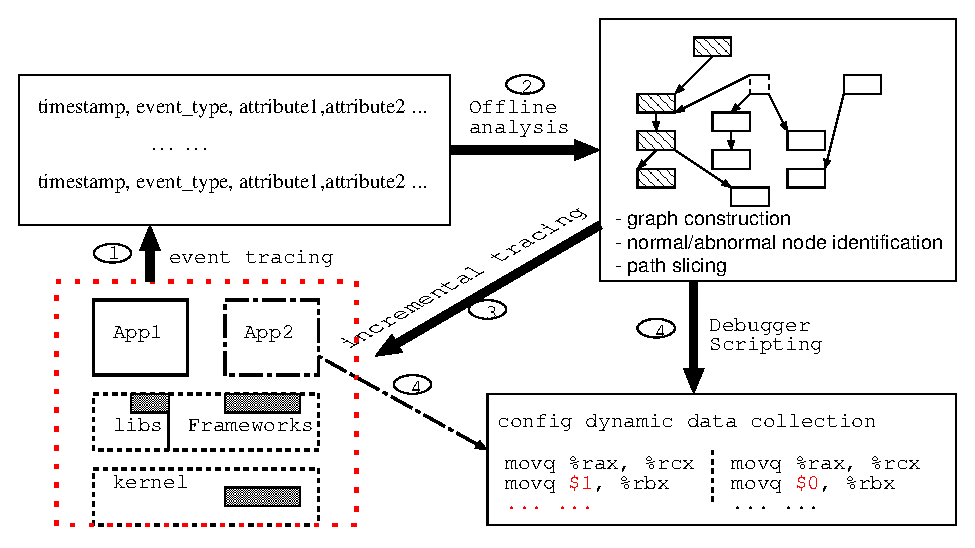
\includegraphics[width=1.0\linewidth]{ArgusOverview.eps}
    \caption{Dedign Overview}
    \label{fig:argus-overview}
\end{figure}

\subsection{Use Cases}

\xxx can be used in two primary ways:
\begin{enumerate}
    \item \xxx can continuously run live in the background and collect full
    system logs. The user works as usual until a crash or performance issue is
    observed.

    \item The user can begin with a reproducible performance issue, no matter how often it appears, and collect
    logs in two situations: a) a baseline situation where the program runs
    normally, and b) a spinning situation that exposes the performance issue.

\end{enumerate}
For a simple issue, like a rare segmentation fault, just having \xxx's lightweight logs may be enough to perform a diagnosis.
However, in most cases, \xxx will need to be used interactively, so the user needs to be able to
%restart the affected application and
reproduce the problem on demand.
The user can request more detailed logs in several ways, then reproduce the problem, and gather enough data to narrow in even further on the issue.
The general process for interactive debugging with \xxx is as follows:
\begin{enumerate}
    \item First, the user finds the node \emph{$N_{spin}$} in the \xxx graph
    that corresponds to a hanging thread of execution. The user may leverage
    the system clock time to search for events (\eg, keystrokes).

    \item Next, the user attempts to find the node in the normal case that
    corresponds with $N_{spin}$. There will likely be many possible candidates
    at first, so the user can narrow in on specific nodes and gather more
    detailed information in that area of the program.

    \item Now, with knowledge of $N_{spin}$ and (a small number of) matching
    nodes in the normal graph, the user performs a backward slice through the
    graphs to attempt to find the defining difference between the cases. This
    difference should accurately predict whether a given log represents a
    normal or spinning case, and usually indicates quite directly the root
    cause. As before, additional information may need to be collected from
    certain points in the program to be able to distinguish between the cases.

\end{enumerate}
As shown in Figure XXX, the user's main operations are a) inspection of
the graph with our toolkits, b) performing slicing on the graph to show dependent nodes, c)
selecting a graph node to gather more information about, and d) comparing graph
slices between normal and spinning cases.
